\documentclass[11pt]{beamer}
\usetheme{Warsaw}
\usepackage[utf8]{inputenc}
\usepackage{amsmath}
\usepackage{amsfonts}
\usepackage{amssymb}
\usepackage{graphicx}
\usepackage{booktabs}
\usepackage{listings}
\lstdefinelanguage{scala}{
  morekeywords={abstract,case,catch,class,def,%
    do,else,extends,false,final,finally,%
    for,if,implicit,import,match,mixin,%
    new,null,object,override,package,%
    private,protected,requires,return,sealed,%
    super,this,throw,trait,true,try,%
    type,val,var,while,with,yield},
  otherkeywords={=>,<-,<\%,<:,>:,\#,@},
  sensitive=true,
  morecomment=[l]{//},
  morecomment=[n]{/*}{*/},
  morestring=[b]",
  morestring=[b]',
  morestring=[b]"""
}

\usepackage{color}
\definecolor{dkgreen}{rgb}{0,0.6,0}
\definecolor{gray}{rgb}{0.5,0.5,0.5}
\definecolor{mauve}{rgb}{0.58,0,0.82}

\lstset{frame=tb,
  language=scala,
  aboveskip=3mm,
  belowskip=3mm,
  showstringspaces=false,
  columns=flexible,
  basicstyle={\small\ttfamily},
  numbers=none,
  numberstyle=\tiny\color{gray},
  keywordstyle=\color{blue},
  commentstyle=\color{dkgreen},
  stringstyle=\color{mauve},
  frame=single,
  breaklines=true,
  breakatwhitespace=true
  tabsize=3
}

\usepackage{algpseudocode}
\usepackage{algorithm}
\algnewcommand\algorithmicforeach{\textbf{for each}}
\algdef{S}[FOR]{ForEach}[1]{\algorithmicforeach\ #1\ \algorithmicdo}

\author{Rodrigo Raya}
\title[Tactic and (co)algebraic reasoning \hspace{25mm} \insertframenumber/\inserttotalframenumber]{Tactic and (co)algebraic reasoning}
\institute[EPFL]
{
  École Polytechnique Fédéral de Lausanne
  \medskip \\
  \textit{}
}
\date{\today} 

\definecolor{Jaguar}{HTML}{262731} 
\definecolor{ChetwodeBlue}{HTML}{6b77ad}
\renewenvironment<>{theorem}[1][\undefined]{
	\begin{actionenv}#2
		\ifx#1\undefined
		\def\insertblocktitle{Theorem}%
		\else
		\def\insertblocktitle{Theorem ({\em#1})}%
		\fi
		\par
		\mode<presentation>{%
			\setbeamercolor{block title}{fg=white,bg=Jaguar!80}
			\setbeamercolor{block body}{fg=black,bg=ChetwodeBlue!10}
		}%
		\usebeamertemplate{block begin}\em}
	{\par\usebeamertemplate{block end}\end{actionenv}}
	
\renewenvironment<>{example}[1][\undefined]{
	\begin{actionenv}#2
		\ifx#1\undefined
		\def\insertblocktitle{Example}%
		\else
		\def\insertblocktitle{Example ({\em#1})}%
		\fi
		\par
		\mode<presentation>{%
			\setbeamercolor{block title}{fg=white,bg=Jaguar!80}
			\setbeamercolor{block body}{fg=black,bg=ChetwodeBlue!10}
		}%
		\usebeamertemplate{block begin}\em}
{\par\usebeamertemplate{block end}\end{actionenv}}	

\usepackage[backend=bibtex, style=numeric]{biblatex}
\addbibresource{references.bib}

\setbeamertemplate{headline}{}
\AtBeginSection[]
{
 \begin{frame}<beamer>
 \tableofcontents[currentsection]
 \end{frame}
}

% Remove foot annotations
\setbeamertemplate{footline}[frame number]{}
\setbeamertemplate{navigation symbols}{}
\setbeamertemplate{footline}{}

% Graphics
\usepackage{tikz-cd}

% Code listings
\usepackage{listings}


\begin{document}

\begin{frame}
\titlepage
\end{frame}

\section{}
\begin{frame}{Overview}
 \tableofcontents
 
\vspace{0.5cm} 

\end{frame}

\begin{frame}{Goal}
\begin{itemize}
	\setlength\itemsep{2em}
	\item How can I design new proof methods?
	\item What are some fancier proof methods?
\end{itemize}
\end{frame}

\section[]{Tactical reasoning}

\begin{frame}{Why tactics}
\begin{itemize}
	\setlength\itemsep{2em}
	\item Widely adopted theorem proving methodology. 
	\item Introduced by Milner in the Edinburgh LCF proof assistant.
	\item Isabelle provides them using three abstraction layers: Isabelle/ML, Isabelle/Isar and Eisbach.
	\item Here: Isabelle/ML. See report for technicalities.
\end{itemize}
\end{frame}

\begin{frame}{Tactical theorem proving vs Isabelle/Isar}
\begin{figure}
	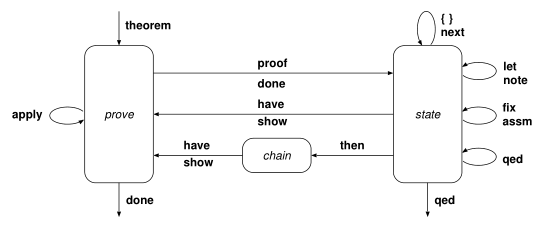
\includegraphics[scale=0.65]{img/isar.png} 
	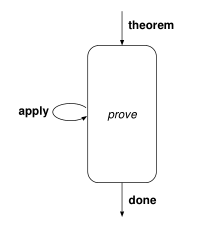
\includegraphics[scale=0.65]{img/tactics.png}
\end{figure}
\end{frame}

\begin{frame}{Demo I}
\begin{itemize}
	\setlength\itemsep{2em}
	\item Hales.thy: \textit{associativity} lemma, local\_setups, concrete\_assoc.
	\item Goal is to prove: \[
	(p_1 \oplus_i p_2) \oplus_j p_3 = p_1 \oplus_k (p_2 \oplus_l p_3)
	\] where $i,j,k,l \in \{0,1\}$ and $\oplus_0,\oplus_1$ are well-defined operations on elliptic curves points.
	\item Good example for the section on structured proofs in the Isabelle Cookbook.
	\item A challenging part (requires debugging): deduce what the rewrite tactic does internally.
\end{itemize}
\end{frame}

\begin{frame}{Demo II}
\begin{itemize}
	\item Experiment3.thy: rewrite sine expressions whose arguments contain sums of multiples of $\pi$.
\end{itemize}

	\begin{enumerate}
	\item Define SIN\_SIMPROC\_ATOM x n = x + of\_int n * pi.
	\item Write a conversion sin\_atom\_conv rewriting of\_int n * pi to SIN\_SIMPROC\_ATOM 0 n and everything else to SIN\_SIMPROC\_ATOM x 0. 
	\item Write a conversion that descends through +, applies sin\_atom\_conv to every atom, and then applies some kind of combination rule like:
	
	SIN\_SIMPROC\_ATOM x1 n1 + SIN\_SIMPROC\_ATOM x2 n2 = 
	SIN\_SIMPROC\_ATOM (x1 + x2) (n1 + n2).
	\item In the end, I have rewritten the original term to the form sin (SIN\_SIMPROC\_ATOM x n), and then I apply some suitable rule to that.
\end{enumerate}
\end{frame}

\section[]{(Co)algebraic reasoning}

\begin{frame}[fragile]{Some categorical notions}
Let $F: Set \to Set$ be a functor.

\settowidth{\leftmargini}{\usebeamertemplate{itemize item}}
\addtolength{\leftmargini}{\labelsep}
\begin{itemize}
\item An \textbf{$F$-algebra} is a set $A$ with a structure mapping $\alpha: F(A) \to A$.
\item $f$ is an \textbf{$F$-homomorphism} between $(A,\alpha)$ and $(B,\beta)$ if this diagram commutes: 

\begin{tikzcd}
F(A) \arrow[d, "\alpha"] \arrow[r, "F(f)"] & F(B) \arrow[d, "\beta"] \\
A \arrow[r, "f"] & B 
\end{tikzcd}

\item \textbf{$Set^F$} is the category formed with $F$-algebras and $F$-homomorphisms.
\item A \textbf{subalgebra} of $\mathcal{A} = (A,s)$ is $S \subseteq A$ with $\beta_S:F(S) \to S$ where the inclusion $i: S \to A$ is a $F$-homomorphism.
\item An \textbf{initial $F$-algebra} is an initial object in $Set^F$. It is unique up to isomorphism. The structure mapping is an isomorphism \textbf{(Lambeck)}.
\end{itemize}
\end{frame}
  
\begin{frame}[fragile]
\settowidth{\leftmargini}{\usebeamertemplate{itemize item}}
\addtolength{\leftmargini}{\labelsep}
\begin{itemize}
\item A relation $R \subseteq S \times T$ is an \textbf{$F$-congruence} if there exists an $F$-algebra structure $(R,\gamma)$ such that the projections $\pi_i$ are $F$-homomorphisms:

\begin{tikzcd}
F(S) \arrow[d, "\alpha"] & F(R) \arrow[l, "F(\pi_1)",swap] \arrow[d, "\gamma",dashed] \arrow[r, "F(\pi_2)"] & F(T) \arrow[d, "\beta"]\\
S  & R \arrow[l, "\pi_1"] \arrow[r, "\pi_2",swap] &  T
\end{tikzcd}

\item By reversing arrows: $F$-coalgebra, coalgebra homomorphism, category $Set_F$, terminal $F$-coalgebra, $F$-bisimulation. 

\item Diagonal of a set: $\Delta(A) = \{(a,a). a \in A\}$

\item \textbf{Induction}: congruences on initial algebras contain $\Delta$.
\item \textbf{Coinduction}: bisimulations on final coalgebras contain $\Delta$.
\item Mathematical induction, streams (co)induction and least (greatest) fixed points characterizations are easy to derive.
\end{itemize}
\end{frame}

\begin{frame}{Functional programming and (co)algebras}
To stress the capabilities of this model, note: \\

\begin{table}
	\begin{center}
		\begin{tabular}{| r | c | l |}
			\hline
			Concept & Category theory & Functional programming \\ \hline
			Datatype & Initial algebra  & 
			\raisebox{-0.8\totalheight}{
				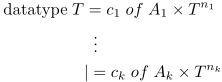
\includegraphics[scale=0.55]{img/datatype.png}
			}
			\\ \hline
		    Iteration & 
			\raisebox{-0.5\totalheight}{
				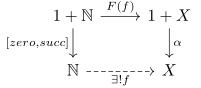
\includegraphics[scale=0.55]{img/initiality.png}
			} &
			\begin{tabular}{@{}c@{}} $f(0) = \alpha(*)$ \\ $f(x+1) = \alpha(f(x))$ \end{tabular}
			\\ \hline
			Recursion & 
			\raisebox{-0.5\totalheight}{
				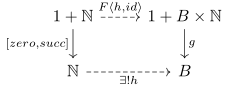
\includegraphics[scale=0.55]{img/primitive.png}
			} &
			\begin{tabular}{@{}c@{}} $h(0) = g_1(*)$ \\ $h(succ(n)) = g_2(h(n), n)$ \end{tabular}
			\\ \hline
			Case analysis &
			\raisebox{-0.5\totalheight}{
				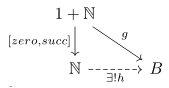
\includegraphics[scale=0.55]{img/case.png}
			} &
			\begin{tabular}{@{}c@{}} $h(0) = g_1(*)$ \\ $h(succ(n)) = g_2(n)$ \end{tabular} \\
			\hline
		\end{tabular}
	\end{center}
\end{table}
\end{frame}

\begin{frame}{Existence of initial algebras}
\textbf{Theorem: }

Let $\mathcal{C}$ be a category with initial object $0$ and colimits for any $\omega$-chain. If $F: \mathcal{C} \to \mathcal{C}$ preserves the colimit of the initial $\omega$-chain, then the initial $F$-algebra is $\mu(F) = \text{colim}_{n < \omega} F^n 0$.

\textbf{Corollary: }

Any polynomial functor on $Set$ admits an initial algebra. \\ 

\textbf{In Isabelle}:

\begin{itemize}
	\item Arbitrary limits require reasoning about infinite type families, which goes beyond HOL capabilities.
	\item This does not include functors of interest: finite powerset ('a fset), countable powerset ('a cset), finite multisets ('a multiset) or discrete probability distributions ('a pmf). Example: datatype 'a tree = Node 'a ('a tree fset)
	
	\item There exist results for bounded endofunctors. Both approaches are related by transfinite induction. 
\end{itemize}
\end{frame}

\begin{frame}{Isabelle approach}
\settowidth{\leftmargini}{\usebeamertemplate{itemize item}}
\addtolength{\leftmargini}{\labelsep}
\begin{itemize}
\item HOL as a category: universe of types $U$ as objects + functions between types as morphisms. 
\item A functor is a type constructor $(\alpha_1,\ldots,\alpha_n)F$ together with a mapping: \[\text{Fmap}: \overline{\alpha} \to \overline{\beta} \to \overline{\alpha} F \to \overline{\beta} F\] such that $\text{Fmap} \; \text{id} = \text{id}$ and $\text{Fmap} (\overline{g} \circ \overline{f}) = \text{Fmap} \, \overline{g} \circ \text{Fmap} \, \overline{f}$.
\item An n-ary bounded natural functor is a tuple $($F, Fmap, Fset, Fbd$)$ where:

\begin{itemize}
	\item $F$ is an n-ary type constructor.
	\item $\text{Fmap}: \overline{\alpha} \to \overline{\beta} \to \overline{\alpha} F \to \overline{\beta} F$
	\item $\forall i \in \{1,\ldots,n\}.$ Fset$_i: \overline{\alpha}F \to \alpha_i \text{ set}$
	\item Fbd is an infinite cardinal number.
\end{itemize}

satisfying the following:

\begin{itemize}
	\item (F,Fmap) is a binary functor.
	\item (F,Fmap) preserves weak pullbacks.
	\item The following cardinal bound conditions hold:
	
	$\forall x : \overline{\alpha} F, i \in {1,\ldots,n}. |\text{Fset}_i \, x | \le \text{Fbd}$
\end{itemize}
\end{itemize}
\end{frame}

\begin{frame}
\settowidth{\leftmargini}{\usebeamertemplate{itemize item}}
\addtolength{\leftmargini}{\labelsep}
\begin{itemize}
	\item $\forall a \in \text{Fset}_i \, x,  i \in \{1,\ldots,n\}. f_i \, a = g_i \, a \implies \text{Fmap} \, \overline{f} \, x = \text{Fmap} \, \overline{g} \, x$
	\item Fset$_i: \overline{\alpha}F \to \alpha_i \text{ set}$ is a natural transformation from:
	
	$((\alpha_1,\ldots,\alpha_{i-1},\textunderscore,\alpha_{i+1},\ldots,\alpha_n)F, \text{Fmap})$ to $(\text{set}, \text{image})$.
\end{itemize}

\textbf{Shape and content intuition} 

\settowidth{\leftmargini}{\usebeamertemplate{itemize item}}
\addtolength{\leftmargini}{\labelsep}
\begin{itemize}
\item The definition of natural transformation for the inclusion mapping $f = i$ gives $\text{Fmap} \, i = i$. 
\item So inclusion lifts to the inclusion.
\item If $(A,t)$ is a $F$-subalgebra of $(B,s)$, then the inclusion $i: A \to B$ is an $F$-algebra homomorphism and $\text{Fmap} \, i = i$.
\item So the subalgebra equation simplifies to $s \circ i = i \circ t$ which implies that $t = s|_{F(A)}$.
\item Thus, for a BNF, a subalgebra can be given by a subset together with a particular restriction of the structure mapping.
\end{itemize}
\end{frame}

\begin{frame}{Constructing the initial algebra: minimal algebra}
\settowidth{\leftmargini}{\usebeamertemplate{itemize item}}
\addtolength{\leftmargini}{\labelsep}
\begin{itemize}
	\setlength\itemsep{2em}
\item Let $\mathcal{A}=(A,s)$ be an $F$-algebra. 

Set $M_s = \bigcap_{B. (B,s|_B) \text{is a subalgebra of (A,s)}} B$ then: \[\mathcal{M}(\mathcal{A}) = \Big(M_s,s \Big|_{M_s} \Big)\] is the $F$-subalgebra generated by $\emptyset$. 

\item We call it the minimal algebra generated by $\mathcal{A}$.
\item $\mathcal{M}(\mathcal{A})$ is said to be the subalgebra generated by $\emptyset$ in the sense that it is the intersection of all subalgebras containing $\emptyset$.
\end{itemize}
\end{frame}

\begin{frame}{Constructing the initial algebra: minimal algebra lemma}
\textbf{Lemma:}

There exists at most one morphism from $\mathcal{M}(\mathcal{A})$ to any other $F$-algebra $(Y,t)$.

\textbf{Proof:}

Since, if $f,g$ are two such morphisms, we can show that: $$B = \mathcal{M}(\mathcal{A}) \cap \{x \in \mathcal{A}. f(x) _= g(x)\}$$ is a $F$-subalgebra of $\mathcal{A}=(A,s)$. Indeed, by our remarks, it suffices to note that $M_s \cap \{x \in \mathcal{A}. f(x) _= g(x)\} \subseteq M_s$ and consider the structure map $s|_B$. This leads to a subalgebra of $\mathcal{M}(\mathcal{A})$ which can be naturally seen as a subalgebra of $\mathcal{A}$. By definition of $\mathcal{M}(\mathcal{A})$, $M_s \subseteq B$ and thus $\forall x \in M_s. f(x) = g(x)$. Thus, $f = g$.
\end{frame}

\begin{frame}{Construction of the initial algebra: naive approach}
\begin{enumerate}
	\item Set $\mathcal{R} = \prod \{\mathcal{A}. \mathcal{A} \text{ is an algebra}\}$.
	\item Given an algebra $\mathcal{A}$, note $h$ the projection morphism from $\mathcal{R}$ to $\mathcal{A}$.
	\item Then $h|_{\mathcal{M}(\mathcal{R})}$ is the unique morphism between $\mathcal{M}(\mathcal{R})$ and $\mathcal{A}$.
	\item Since the construction does not depend on the chosen algebra $\mathcal{A}$,  $\mathcal{M}(\mathcal{R})$ is the desired initial algebra.
\end{enumerate}

\textbf{Problems in HOL:}

\begin{enumerate}
	\item One cannot quantify over infinite type collections. 
	\item The product of the carrier sets of all algebras, fails itself to be a set.
\end{enumerate}
\end{frame}

\begin{frame}{Construction of the initial algebra: for a fixed algebra}
\settowidth{\leftmargini}{\usebeamertemplate{itemize item}}
\addtolength{\leftmargini}{\labelsep}
\begin{itemize}
		\setlength\itemsep{2em}
	\item Given an $F$-algebra $\mathcal{A}$ we know that there exists at most one morphism $\mathcal{M}(\mathcal{A}) \to \mathcal{A}$. But from the shape and content intuition, for bounded natural functors, the inclusion is one such morphism. So there is exactly one morphism $g: \mathcal{M}(\mathcal{A}) \to \mathcal{A}$.
	\item Goal: give a set of algebras $\mathcal{R}$ such that from $\mathcal{R}$ there is a unique morphism to any $\mathcal{M}(\mathcal{A})$. 
	\item Strategy: find a sufficiently large type $T_0$ such that its cardinality is an upperbound for any $\mathcal{A}$. 
\end{itemize}

\end{frame}

\begin{frame}{Construction of the initial algebra: for an arbitrary algebra}

\[|A| \le_o (r :: 'b \, \text{set}) \implies \exists f \; B::'b \; \text{set}. \text{bij\_betw} f \; B \; A \;\; (ex\_bij\_betw) \]

If we can bound the cardinality of a set by some ordinal then the set has a bijective representation on the carrier of the wellorder inducing the ordinal. 

For any algebra $\mathcal{A}$, with $M$ the carrier of $\mathcal{M}(\mathcal{A})$, $|M| \le_o 2  \wedge_c k$. The package witnesses a type $T_0$ with this cardinality and sets: \[\mathcal{R} = \prod \{\mathcal{A}. \mathcal{A} = (A,s) \text{ is an algebra with structure map } s: T_0 F \to T_0 \}\] By means of $ex\_bij\_betw$, the minimal algebras $\mathcal{M}(\mathcal{A})$ have isomorphic representants on a component of $\mathcal{R}$. Thus, the corresponding projection from the product to $\mathcal{M}(\mathcal{A})$ restricted to $\mathcal{M}(\mathcal{R})$ is the unique morphism  $f$ between the two. 

Then, $f \circ g: \mathcal{M}(\mathcal{R}) \to \mathcal{A}$ is a suitable morphism. One shows it is the unique morphism between the two with a similar argument as the previous lemma. 
\end{frame}

\section{Conclusion and references}

\begin{frame}{Conclusion}
\begin{itemize}
			\setlength\itemsep{2em}
	\item We have explored the Isabelle/ML: including tactics, parsing of specifications, new proof commands and definitional packages. 
	\item We have seen a practical use of category theory in a real-world tool formalizing (co)datatypes as bounded natural functors. 
	\item Next natural step: explore the logic foundations of several proof assistants. 
\end{itemize}
\end{frame}

\begin{frame}[allowframebreaks]{References}
\nocite{*}
\printbibliography
\end{frame}





\end{document}